\newif\ifSpringerFormat
\IfFileExists{sn-jnl.cls}{
  \SpringerFormattrue
  \documentclass[pdflatex,sn-mathphys-num]{sn-jnl}
}{
  \documentclass[10pt,a4paper]{article}
  \usepackage[textwidth=31pc,textheight=194.25mm]{geometry}
  \usepackage[T1]{fontenc}
  \usepackage[numbers,sort&compress]{natbib}
  \usepackage[hidelinks]{hyperref}
  \typeout{Preview mode: sn-jnl.cls is unavailable; Springer formatting is not active.}
}

\usepackage{amsmath,amssymb,amsthm}
\usepackage{booktabs,tabularx,array}
\usepackage{graphicx}
\usepackage{xurl}
\usepackage{microtype}
\IfFileExists{sn-jnl.cls}{}{\usepackage[title]{appendix}}
\usepackage{tikz}
\usetikzlibrary{arrows.meta,positioning,fit,backgrounds,shapes.geometric,calc}
\newtheorem{proposition}{Proposition}
\newtheorem{assumption}{Assumption}
\newtheorem{lemma}{Lemma}[section]
\newcommand{\Prob}{\mathbb{P}}
\newcommand{\Expect}{\mathbb{E}}
\newcommand{\ind}{\mathbf{1}}
\newcommand{\TV}{\operatorname{TV}}
\newcommand{\FPR}{\operatorname{FPR}}
\newcommand{\TPR}{\operatorname{TPR}}
\newcommand{\calD}{\mathcal{D}}
\newcommand{\calA}{\mathcal{A}}
\newcommand{\calF}{\mathcal{F}}
\newcommand{\calH}{\mathcal{H}}
\newcolumntype{Y}{>{\raggedright\arraybackslash}X}
\raggedbottom

\ifSpringerFormat
  \makeatletter
  \def\email#1{\global\advance\emailcnt by 1\relax%
    \if@corauemail%
      \g@addto@macro\corrauthemail{#1; }%
    \else%
      \g@addto@macro\authemail{#1; }%
    \fi}
  \hypersetup{colorlinks=false,hidelinks}
  \makeatother
\fi

\makeatletter
\ifSpringerFormat
  \g@addto@macro\ps@headings{\let\@oddhead\@empty\let\@evenhead\@empty}
  \g@addto@macro\ps@titlepage{\let\@oddhead\@empty\let\@evenhead\@empty}
  \pagestyle{headings}
\fi
\makeatother

\begin{document}

\newcommand{\proposaltitle}{Sequential Testing for AI Text Detection: From Sample-Complexity Bounds to Conformal Guarantees}
\newcommand{\proposalsubtitle}{A research proposal for cost-aware, within-document method selection}
\newcommand{\proposalkeywords}{AI-generated text detection, sequential testing, conformal calibration, sample complexity, adaptive method selection, false-positive control}

\newcommand{\proposalabstract}{We propose a protocol for deciding how much text to inspect and which detector to run before flagging a document for review or stopping without an alert. Researchers have developed sample-complexity bounds, length-aware conformal calibration, and sequential betting tests for document streams. We study adaptive inspection within one document, accounting for repeated looks and detector switches under a shared false-alert target. We distinguish independent-document sample counts from token budgets and measure detection power alongside error control. We use two finite-sample constructions: a registered family of prefix--detector tests with fixed error allocation, and calibration of the complete-path maximum of a frozen adaptive policy. Under document-level exchangeability, we prove marginal control of any false alert along the allowed inspection path; neither proof requires independent tokens. We quantify the calibration counts needed for rejection and set out a power--cost evaluation on public benchmarks. The experiments will compare matched-error procedures under generator and domain holdouts, paraphrasing, and mixed authorship, with subgroup audits where metadata permit them. We report historical pilot measurements under this joint criterion; the designed multi-corpus study has not been completed. In the pilot, Construction B met the joint cost-and-power criterion in fourteen of eighteen cells, although most of those passes occurred where both policies had near-zero power and the cost limb alone decided the outcome. The proposed study will test whether adaptive inspection saves computation at comparable power and identify the conditions under which those savings fail.}

\ifSpringerFormat
  \title[Sequential Testing for AI Text Detection]{\proposaltitle}
  \subtitle{\proposalsubtitle}
  \author*[1]{\fnm{Charlie Margaret} \sur{Balagtas}}
  \email{corresponding.author@replace-before-submission.edu.ph}
  \author[1]{\fnm{Michael Joshua} \sur{Buluran}}
  \author[1]{\fnm{Jeff Roel} \sur{Durmiendo}}
  \author[1]{\fnm{Rizzette E.} \sur{Lopez}}
  \affil[1]{\orgname{Bulacan State University}}
  \abstract{\proposalabstract}
  \keywords{\proposalkeywords}
  \maketitle
\else
  \title{\proposaltitle\\[0.5em]{\large\proposalsubtitle}}
  \author{Charlie Margaret Balagtas\,$^*$ \and Michael Joshua Buluran
    \and Jeff Roel Durmiendo \and Rizzette E. Lopez}
  \date{\small Content preview: Springer class unavailable\\
    \small $^*$Corresponding author e-mail to be supplied at submission}
  \maketitle
  \begin{center}
    Bulacan State University
  \end{center}
  \begin{abstract}
    \proposalabstract
  \end{abstract}
  \noindent\textbf{Keywords:} \proposalkeywords
\fi

\section{Introduction and proposed contribution}\label{sec:intro}

Researchers screening text must choose an inspection budget and decide whether another detector call justifies its cost. They can use probability-curvature scores from DetectGPT and Fast-DetectGPT or contrasting-model scores from Binoculars \citep{mitchell2023,bao2024,hans2024}. To preserve a false-alert target while inspecting additional prefixes or switching detectors, they need error accounting for the whole decision path. Published results for a fixed scoring procedure do not establish that guarantee.

We will test whether adaptive stopping and detector selection reduce expected inspection cost at a prespecified probability of any false alert on a human document. We interpret a rejection as a \emph{screening alert against a specified human-reference distribution}. Human authors can produce text outside that reference population, so an alert cannot establish machine authorship or misconduct. We retain an insufficient-evidence status for documents that receive no alert.

Zhu et al.\ introduce length-aware multiscaled conformal prediction (MCP), and Chen and Wang develop sequential betting tests for streams of texts \citep{zhu2025,chen2025}. We build on this work to study \emph{within-document} inspection with detectors of different computational costs. Our claims require limits: useful token budgets depend on distributional separation, and a fixed-inspection conformal guarantee does not justify repeated testing at the same nominal level.

We will develop and evaluate two components:
\begin{enumerate}
\item A detector-selection protocol with one document-level false-alert target. We treat tokens as the inspection budget and prove validity through fixed error allocation or complete-policy calibration. We use these elementary constructions as baselines.
\item A power--cost evaluation of adaptive inspection, including the effects of limited calibration data, weak separation, and distribution shift.
\end{enumerate}

Fig.~\ref{fig:workflow} shows the end-to-end workflow from split construction through offline calibration to online screening. Fig.~\ref{fig:constructions} contrasts the two validity constructions on the same inspection route.

\begin{figure}[t]
\centering
\begin{tikzpicture}[
  font=\footnotesize,
  stage/.style={draw, rounded corners=3pt, align=center, inner sep=5pt, fill=black!3},
  band/.style={draw, rounded corners=4pt, align=left, inner sep=5pt, fill=black!2},
  step/.style={draw, rounded corners=2pt, align=center, inner sep=3.5pt, fill=white},
  arr/.style={-{Stealth[length=4.5pt]}, thick},
  note/.style={font=\scriptsize\itshape, text=black!55, align=left}
]
  \node[band, text width=0.94\textwidth] (dev) {
    \textbf{1 · Development (frozen)}\quad
    corpus splits (lineage-grouped)
    \;$\to$\;
    score orientation, routing $\pi$, weights $w_a$
    \;$\to$\;
    futility rule and cost model\\[1pt]
    {\scriptsize\itshape No calibration ranks or test document used here.}
  };
  \node[band, text width=0.94\textwidth, below=12pt of dev] (cal) {
    \textbf{2 · Human calibration (offline)}\quad
    $H_1,\ldots,H_m$
    \;$\to$\;
    A: score all registered actions
    \;\textbar\;
    B: replay full route $\to M_\pi(H_i)$\\[1pt]
    {\scriptsize\itshape Store ranks / path maxima; resolution floor $m\geq\lceil1/(\alpha w_a)\rceil-1$.}
  };
  \node[band, text width=0.94\textwidth, below=12pt of cal] (scr) {
    \textbf{3 · Online screening (test document $X$)}\\[3pt]
    \texttt{low-cost \(a_1\)}\;$\to$\;
    route / extend \(b_k\)\;$\to$\;
    switch detector\;$\to$\;
    futility or cap\;$\to$\;
    no alert\\[3pt]
    {\scriptsize\itshape Alert if $p_a\leq\alpha w_a$ or $p_t^{\rm path}\leq\alpha$; otherwise stop on futility, end of evidence, or resource cap.}
  };
  \draw[arr] (dev.south) -- (cal.north);
  \draw[arr] (cal.south) -- (scr.north);
  \node[note, text width=0.94\textwidth, below=6pt of scr]
    {Exchangeability is at the document level; tokens inside a document may be arbitrarily dependent. Outputs: \emph{flag for review} or \emph{no alert at this budget} (insufficient evidence).};
\end{tikzpicture}
\caption{End-to-end screening workflow. Development freezes routing, weights, and the futility rule without touching calibration ranks. Offline calibration scores every registered action (Construction A) and replays the complete frozen route to obtain path maxima (Construction B). Online screening executes a prefix--detector action, checks the appropriate rank against its boundary, and either alerts or continues under the routing and futility rules}
\label{fig:workflow}
\end{figure}

\begin{figure}[t]
\centering
\begin{tikzpicture}[
  font=\footnotesize,
  box/.style={draw, rounded corners=2pt, align=center, inner sep=4pt},
  arr/.style={-{Stealth[length=4pt]}, thick},
  good/.style={box, fill=black!3},
  lab/.style={font=\scriptsize\itshape, text=black!55}
]
  \node[box, fill=black!8] (p1) {\(b_1{=}128\)};
  \node[box, fill=black!8, right=10pt of p1] (p2) {\(b_2{=}256\)};
  \node[box, fill=black!8, right=10pt of p2] (p3) {\(b_3{=}512\)};
  \node[box, fill=black!8, right=10pt of p3] (p4) {\(b_4{=}1024\)};
  \draw[arr] (p1) -- (p2);
  \draw[arr] (p2) -- (p3);
  \draw[arr] (p3) -- (p4);
  \node[lab, above=4pt of p1.west, anchor=west] {shared inspection path (detector may switch at each step)};

  \node[good, below=16pt of $(p1.south)!0.5!(p2.south)$, text width=0.42\textwidth] (ca) {
    \textbf{Construction A · error budget}\\
    Each executed action has \(\alpha_a=\alpha w_a\).\\
    Alert if any \(p_a\leq\alpha_a\).\\
    {\scriptsize Union bound \(\Rightarrow\) \(\Prob(\text{any alert})\leq\sum\alpha_a\leq\alpha\).\\
    Active subset sized by \(\lfloor\alpha(m+1)\rfloor\).}
  };
  \node[good, below=16pt of $(p3.south)!0.5!(p4.south)$, text width=0.42\textwidth] (cb) {
    \textbf{Construction B · path maximum}\\
    Calibrate \(M_\pi=\max_t g_a(S_a)\) on complete routes.\\
    Alert at first \(t\) with \(p_t^{\rm path}\leq\alpha\).\\
    {\scriptsize Partial max \(\leq\) complete max \(\Rightarrow\) early stop inherits terminal rank.}
  };

  \draw[arr, dashed] (p2.south) -- (ca.north);
  \draw[arr, dashed] (p3.south) -- (cb.north);
  \node[lab, right=4pt of p4.east, anchor=west] {cap};
\end{tikzpicture}
\caption{The two validity constructions on the same prefix route. Construction A splits a single \(\alpha\) across registered actions and relies on a union bound over whatever subset is executed. Construction B freezes one route, calibrates the complete-path maximum once, and lets partial-path ranks inherit the terminal guarantee, so early stopping does not spend error across looks}
\label{fig:constructions}
\end{figure}

\section{Literature validation and scope of novelty}\label{sec:literature}

\subsection{Detectability and sample complexity}

Chakraborty et al.\ derive sample-complexity results under stated settings, including an independent and identically distributed (i.i.d.) formulation \citep{chakraborty2024}. We use their analysis to motivate evidence budgeting; applying it to word counts would require assumptions about within-document dependence. Sadasivan et al.\ study detection limits under distributional similarity and adversarial paraphrasing \citep{sadasivan2025}. Researchers can gain power from independent evidence against a fixed separated alternative, yet encounter weak detection when the distributions approach each other or an adversary edits the text. A learned score can discard information that an oracle test would use.

\subsection{Zero-shot detector scores}\label{sec:detectors}

Three zero-shot score families motivate the registered detector set (Table~\ref{tab:detectors}). We summarize their mechanisms, cost profiles, and how each enters our protocol; Fig.~\ref{fig:detectors} contrasts them schematically.

\paragraph*{DetectGPT (probability curvature).}
Mitchell et al.\ perturb a candidate passage with a masked language model \(q_\varphi\), rescore each perturbation under a scoring model \(p_\theta\), and compare the original log-probability to the mean of the perturbed scores \citep{mitchell2023}:
\begin{equation}
 d(x,p_\theta,q_\varphi)=\log p_\theta(x)
 -\Expect_{\tilde x\sim q_\varphi(\cdot\mid x)}[\log p_\theta(\tilde x)].
 \label{eq:detectgpt}
\end{equation}
Machine-generated text tends to sit near a local maximum of the model's probability landscape, so \(d\) is positive under the source model and near zero for human text. Estimating the expectation requires on the order of one hundred perturbation--rescore cycles, which makes DetectGPT an expensive white-box comparator rather than a routine prefix action. On DetectRL, DetectGPT's average AUROC falls well below simpler rank baselines under real-world attacks \citep{wu2024}, consistent with our decision to keep it off the default inspection route.

\paragraph*{Fast-DetectGPT (conditional probability curvature).}
Bao et al.\ replace the perturb--rescore loop with conditional independent sampling \citep{bao2024}. They sample alternative next-tokens from a reference model given the fixed passage, evaluate the conditional probability of the observed continuation in one forward pass, and form a standardized residual
\begin{equation}
 \hat d_x=\frac{\log p_\theta(x)-\tilde\mu}{\tilde\sigma},
 \label{eq:fastdetectgpt}
\end{equation}
where \(\tilde\mu,\tilde\sigma\) are moments of the sampled conditional log-probabilities. The method reports roughly \(75\%\) relative AUROC gains over DetectGPT in both white-box and black-box settings and about a \(340\times\) speedup, because all samples are evaluated in a single predictive distribution rather than through hundreds of model calls. Fast-DetectGPT is therefore a natural optional registered extension: one action can compute the score in a single batched pass, and its cost profile is closer to a single scoring model than to DetectGPT's perturbation pipeline.

\paragraph*{Binoculars (contrastive perplexity ratio).}
Hans et al.\ view the text through two closely related language models \citep{hans2024}. An observer model supplies log-perplexity of the observed tokens; a performer model supplies next-token predictions whose perplexity under the observer is the cross-perplexity. The Binoculars score is the ratio of the two perplexities: machine text written by a similar generator drives the two perplexities toward each other, while human text leaves a larger gap. Without training data or model-specific tuning, Binoculars reports over \(90\%\) detection of ChatGPT text at a false-positive rate of \(0.01\%\) across news, creative writing, and student essays, and remains competitive under domain shift because modern LLMs share architecture and training-corpus structure. The detector needs two forward passes per prefix (observer and performer), so its per-action cost sits between a single likelihood score and DetectGPT's perturbation bank. We register Binoculars as an optional contrasting-model action and profile it under the same prefix budgets as the single-model scores.

\paragraph*{Rank and log-rank baselines.}
Alongside these methods we keep average token rank and log-rank scores, which require only one scoring model and no sampling or second network. On DetectRL, log-rank and rank baselines often match or exceed Fast-DetectGPT under attack \citep{wu2024}, so they remain first-class registered actions rather than merely cheap fallbacks. The stylometric (stop-slop) score is a lexicon hit-count over the inspected prefix; it is a surface signal for routing and reporting, not a substitute for probabilistic evidence.

\begin{table}[t]
\caption{Zero-shot score families used or considered as registered detectors. Costs are qualitative relative orders for one prefix under our planned batching; exact milliseconds are hardware-dependent and will be profiled}\label{tab:detectors}
\small
\begin{tabularx}{\textwidth}{@{}>{\raggedright\arraybackslash}p{0.16\textwidth}Yp{0.14\textwidth}p{0.16\textwidth}@{}}
\toprule
Score family & Mechanism & Model calls per prefix & Role in the protocol \\
\midrule
Likelihood (LL) & Mean per-token log-probability under one scoring LM & 1 & Fixed comparator (\texttt{ll@1024}); registered action \\
Rank / log-rank & Mean token rank or log-rank under one scoring LM & 1 & Registered action (cheap, robust baselines) \\
Binoculars & Observer perplexity / cross-perplexity from a performer pair & 2 & Optional contrasting-model registered action \\
Fast-DetectGPT & Conditional probability curvature via independent token sampling & 1 scoring + 1 sampling batch & Optional registered extension \\
DetectGPT & Marginal probability curvature via mask-fill perturbations & \(\sim100\) perturb--rescore cycles & Expensive comparator; not on the default route \\
Stop-slop (stylometric) & Lexicon hit-rate over the inspected prefix & 0 (string match) & Surface signal / routing feature only \\
\bottomrule
\end{tabularx}
\end{table}

\begin{figure}[t]
\centering
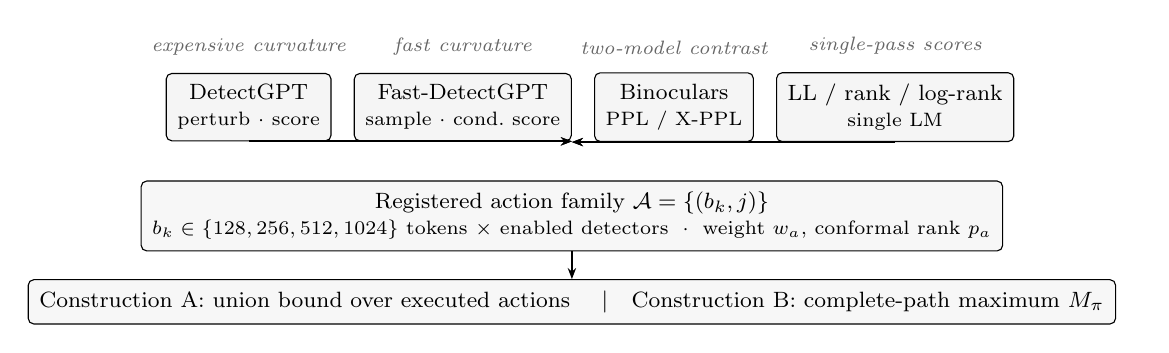
\begin{tikzpicture}[
  font=\footnotesize,
  box/.style={draw, rounded corners=2pt, align=center, inner sep=4pt, minimum height=1.1em},
  det/.style={box, fill=black!4},
  opt/.style={box, densely dashed},
  lab/.style={font=\scriptsize\itshape, text=black!60},
  arr/.style={-{Stealth[length=4pt]}, thick}
]
  \node[det] (dg) {DetectGPT\\ \scriptsize perturb \(\cdot\) score};
  \node[det, right=8pt of dg] (fd) {Fast-DetectGPT\\ \scriptsize sample \(\cdot\) cond.\ score};
  \node[det, right=8pt of fd] (bi) {Binoculars\\ \scriptsize PPL / X-PPL};
  \node[det, right=8pt of bi] (rk) {LL / rank / log-rank\\ \scriptsize single LM};

  \node[lab, above=3pt of dg] {expensive curvature};
  \node[lab, above=3pt of fd] {fast curvature};
  \node[lab, above=3pt of bi] {two-model contrast};
  \node[lab, above=3pt of rk] {single-pass scores};

  \node[box, below=14pt of $(dg.south)!0.5!(rk.south)$, minimum width=0.86\textwidth, fill=black!3]
    (reg) {Registered action family \(\calA=\{(b_k,j)\}\)\\
      \scriptsize \(b_k\in\{128,256,512,1024\}\) tokens \(\times\) enabled detectors \(\;\cdot\;\) weight \(w_a\), conformal rank \(p_a\)};
  \node[box, below=10pt of reg, fill=black!3, minimum width=0.86\textwidth]
    (dec) {Construction A: union bound over executed actions
      \quad\textbar\quad
      Construction B: complete-path maximum \(M_\pi\)};

  \draw[arr] (dg.south) -- (reg.north |- dg.south);
  \draw[arr] (fd.south) -- (reg.north |- fd.south);
  \draw[arr] (bi.south) -- (reg.north |- bi.south);
  \draw[arr] (rk.south) -- (reg.north |- rk.south);
  \draw[arr] (reg.south) -- (dec.north);
  \node[lab, right=2pt of dec.east, anchor=west] {};
\end{tikzpicture}
\caption{Score families and how they enter the registered action family. DetectGPT's marginal curvature needs roughly a hundred perturb--rescore cycles and is held as an expensive comparator; Fast-DetectGPT estimates conditional curvature in one sampling batch; Binoculars contrasts observer and performer perplexities; likelihood and rank scores are single-pass. Each enabled score multiplies the four prefix budgets to form the registered actions that Construction A weights and Construction B freezes into a route}
\label{fig:detectors}
\end{figure}

AdaDetectGPT learns a witness function from training data \citep{zhou2025adadetect}. Its adaptation concerns score learning; our policy selects inspections within a test document after development. We will distinguish these tasks when choosing baselines. A learned score could enter the registered family, but its fixed-decision guarantee would not replace pathwise error accounting.

\subsection{Calibration baselines and sequential evidence}

Zhu et al.\ calibrate detection scores within text-length bins in MCP \citep{zhu2025}. We will use MCP as a fixed-decision calibration baseline. We read its stated rule as assigning a threshold from the length of the submitted text. Selecting the minimum of several prefix-specific \(p\)-values requires an additional bound, which we supply for our proposed inspection rules. We follow the distinction between marginal and calibration-conditional validity in conformal outlier testing \citep{bates2023}.

Wald developed sequential hypothesis tests \citep{wald1945}; Howard et al.\ give time-uniform bounds through nonnegative supermartingales \citep{howard2020}. For AI-text detection, Chen and Wang combine detector scores with sequential betting to make source-level decisions from a stream of texts, with false-positive and expected-detection-time guarantees \citep{chen2025}. We will compare with their method in a separate document-stream experiment. Applying it to adjacent paragraphs would require a new justification for the dependence within a document.

Koning and van Meer induce sequential tests from terminal tests \citep{koning2026anytime}. Construction A applies weighted Bonferroni testing to conformal ranks; Construction B uses an observable lower bound on terminal rejection. We study these implementations for within-document screening and do not claim a new multiple-testing inequality or sequential-test induction principle.

Kirchenbauer et al.\ embed watermarks during generation \citep{kirchenbauer2023}. Xie et al.\ combine watermark evidence with conformal methods to assess permissible versus impermissible AI assistance in educational settings \citep{xie2026}. We restrict this study to passive detection of unwatermarked text and make no claim to originate conformal AI-use decisions. Table~\ref{tab:position} positions these strands against the present proposal.

\begin{table}[t]
\caption{Prior work and the scope of the proposed study}\label{tab:position}
\small
\begin{tabularx}{\textwidth}{@{}>{\raggedright\arraybackslash}p{0.24\textwidth}YY@{}}
\toprule
Research strand & Established relevance & Proposed distinction \\
\midrule
Zero-shot scores \citep{mitchell2023,bao2024,hans2024} & Curvature and contrastive perplexity separate machine from human text at fixed thresholds. & Wrap any enabled score in a pathwise false-alert guarantee under one \(\alpha\). \\
Sample complexity \citep{chakraborty2024} & Detectability depends on evidence and distributional separation. & Translate this motivation into measured power--cost curves without equating tokens with independent samples. \\
Length-aware MCP \citep{zhu2025} & Human-reference calibration adapts thresholds to text length. & Protect a decision across multiple inspected prefixes and switched detectors. \\
Online betting \citep{chen2025} & Error and delay guarantees for sequential source detection. & Study one document with within-text dependence and heterogeneous scoring costs. \\
Conformal outliers \citep{bates2023} & Finite-sample marginal validity and stronger calibration-conditional methods. & Make the guarantee level explicit in an implementable screening workflow. \\
Watermark calibration \citep{xie2026} & Conformal AI-use decisions with watermark evidence. & Restrict the primary study to passive detection without generation-side access. \\
\bottomrule
\end{tabularx}
\end{table}

\subsection{Limits of KS tests on word identifiers}

Researchers use a Kolmogorov--Smirnov (KS) statistic to compare empirical distribution functions of ordered scalar observations. Standard two-sample KS calibration requires independent samples from continuous distributions \citep{scipyks}. Assigning numeric identifiers to words supplies an arbitrary order: a researcher can change the KS statistic by relabeling the same word types. Repeated words create ties, and neighboring tokens are dependent. A standard KS routine on word identifiers therefore lacks the assumptions needed for an authorship test.

We may use a KS-type discrepancy on prespecified scalar scores as a feature, with document-level conformal calibration or permutation calibration under suitable exchangeability. The resulting test concerns the score distributions. We include the raw-word example as a methodological check and attribute it to no named paper.

\section{Statistical target and sampling units}\label{sec:setup}

Let \(X=(W_1,\ldots,W_L)\) denote one complete document, including its length and acquisition metadata. We specify a human-document reference population \(P_0\), with \(X\sim P_0\) under the null, and a family \(\mathcal Q\) of generated or AI-assisted alternatives. Rejecting \(P_0\) cannot identify \(\mathcal Q\), since human populations outside the reference can differ from \(P_0\).

We specify a policy \(\pi\) that selects an inspection extent and detector at each step. We allow stopping with or without an alert, or escalation within a resource limit. We report one of two outcomes:
\begin{enumerate}
\item \emph{Flag for review}: the valid alert boundary has been crossed.
\item \emph{No alert at this budget}: we terminate without crossing and retain an insufficient-evidence status.
\end{enumerate}
We include futility stops in the second output. Certifying human authorship would require a specified alternative-null test and its own error analysis.

Let \(\tau\) be the number of actions executed, \(N_\tau\) the number of distinct document tokens inspected, and \(C_\tau\) total computational cost. These are different quantities: several detectors may rescore the same tokens. The principal validity target is
\begin{equation}
 \Prob_{\calD_{\rm cal},X\sim P_0,\pi}
 \{\text{an alert occurs at any allowed action}\}\leq\alpha.
 \label{eq:target}
\end{equation}
We average over calibration data, a new null document, and policy randomness to obtain \emph{marginal document-level} control. A posterior probability of AI authorship would require a separate probabilistic model. The bound supplies neither a guarantee conditional on each calibration set, length, subgroup, or selected route nor family-wise control over a collection of screened documents.

\begin{assumption}[Development separation and exchangeability]\label{ass:exchange}
All score definitions, model checkpoints, preprocessing, action sets, routing policies requiring frozen calibration, and error weights are fixed using development data \(\calD_{\rm dev}\). Weights may be instantiated by a development-frozen rule that depends only on design parameters (calibration count \(m\), nominal level \(\alpha\)), the registered family, and development-fixed priority order---never on calibration scores or the test document. Conditional on that development information, the human calibration documents \(H_1,\ldots,H_m\) and a new null document \(X\) are exchangeable. Any per-document randomization is applied symmetrically, for example using independent seeds with the same distribution.
\end{assumption}

We impose exchangeability at the \emph{document} level and allow arbitrary token dependence within a document. We must prevent leakage and duplicates across development and calibration splits, and assess shifts between calibration and deployment. For a prespecified domain or length stratum, we require exchangeability within that stratum and replace \(m\) by its calibration count. We will abstain in sparse or unavailable strata unless we can justify a pooled analysis.

\section{From evidence requirements to cost-aware decisions}\label{sec:complexity}

\subsection{Oracle evidence bounds}

For an idealized experiment observing \(n\) independent complete documents from either \(P_0\) or a fixed \(Q\), the minimum sum of type-I and type-II errors over all tests is
\begin{equation}
 \inf_{\phi}\left\{P_0^{\otimes n}(\phi=1)
       +Q^{\otimes n}(\phi=0)\right\}
 =1-\TV(P_0^{\otimes n},Q^{\otimes n}).
 \label{eq:tv}
\end{equation}
We use \(\TV(P,Q)=\sup_B|P(B)-Q(B)|\). For a rejection region \(B\), the error sum is \(1-[Q(B)-P_0(B)]\); we obtain the identity by optimizing over regions. This is an oracle bound for independent replicates, consistent with the distributional-separation limits in the detection literature \citep{chakraborty2024,sadasivan2025}. Applying it to a learned detector would require an analysis of the information retained by its score.

For a simpler score-based illustration, suppose \(Z_1,\ldots,Z_n\in[0,1]\) are independent scores with null mean \(\mu_0\) and alternative mean \(\mu_0+\Delta\), where \(\Delta>0\). If both means are known, the fixed rule \(\bar Z_n\geq\mu_0+\Delta/2\) has each error probability bounded by \(\exp(-n\Delta^2/2)\), by Hoeffding's inequality \citep{hoeffding1963}. Thus a sufficient oracle budget is
\begin{equation}
 n\geq \frac{2}{\Delta^2}
 \max\{\log(1/\alpha),\log(1/\beta)\}.
 \label{eq:oraclebudget}
\end{equation}
We obtain a budget proportional to \(\Delta^{-2}\) under known score means and independent observations. Extending this calculation to our conformal rules would require accounting for mean estimation, score selection, and repeated inspection. Applying it to tokens would require an analysis of their dependence.

\subsection{Empirical token budgets}

For a frozen single-inspection rule using detector \(j\) at token budget \(b\), define a benchmark-specific evidence requirement
\begin{equation}
 b_j^*(Q;\alpha,\beta)
 =\inf\{b:\TPR_{Q,j,b}(\alpha)\geq 1-\beta\},
 \label{eq:empbudget}
\end{equation}
where \(\TPR_{Q,j,b}(\alpha)\) includes the specified calibration procedure. We set the value to infinity if no supported budget meets the target. We will estimate the crossing with uncertainty and report the full power curve, since a learned detector's power need not increase with length.

We will develop the adaptive policy through the empirical constrained problem
\begin{equation}
 \min_{\pi\in\Pi}\Expect_{X\sim R}[C_\tau]
 \quad\text{subject to}\quad
 \FPR_{P_0}(\pi)\leq\alpha,\qquad
 \min_{Q\in\mathcal Q_{\rm dev}}\TPR_Q(\pi)\geq1-\beta.
 \label{eq:objective}
\end{equation}
We specify a workload mixture \(R\), restrict the policy class \(\Pi\), and use development alternatives in \(\mathcal Q_{\rm dev}\). We enforce the first constraint through the validity constructions under their stated assumptions. We fit to the power target during development and evaluate it on untouched alternatives. If we cannot meet it, we will report infeasibility or preregister a revised target before evaluation.

\section{Two valid sequential constructions}\label{sec:methods}

\subsection{Construction A: a registered family with an error budget}

Fix a finite action family \(\calA\). For action \(a=(k,j)\), choose a token budget \(b_k\) and detector \(j\). Compute \(S_a(X)\) from the first \(\min(b_k,L)\) tokens using a fixed rule, with larger values more suspicious. Apply the same mapping to each calibration document, including end-of-document and failure handling. Assign score \(-\infty\) to a detector failure to prevent an alert from that action. Define each action on all documents, including those for which the policy would skip it.

For each action, form a split-conformal upper-tail rank
\begin{equation}
 p_a(X)=\frac{1+\sum_{i=1}^{m}\ind\{S_a(H_i)\geq S_a(X)\}}{m+1}.
 \label{eq:rank}
\end{equation}
Under Assumption~\ref{ass:exchange}, this rank is super-uniform for a new null document. We use the weak inequality for conservative tie handling, following the conformal outlier rank argument \citep{bates2023}.

Choose fixed weights \(w_a\geq0\) with \(\sum_{a\in\calA}w_a\leq1\), and let \(\alpha_a=\alpha w_a\). Use observed scores or ranks to choose a subset of registered actions and their execution order. Issue an alert if an executed action satisfies \(p_a\leq\alpha_a\); no other event authorizes an alert. Keep unused error allocations fixed after observing the test document. Reuse the frozen score or seed when repeating an action. A fresh random replicate requires a separate action and error allocation.

\begin{proposition}[False-alert control under action selection]\label{prop:spending}
Under Assumption~\ref{ass:exchange}, Construction A satisfies \eqref{eq:target}, regardless of dependence between action scores and regardless of adaptive stopping or action selection within the registered family.
\end{proposition}
\begin{proof}
For each fixed action, exchangeability gives \(\Prob_0(p_a\leq\alpha_a)\leq\alpha_a\). The event that the policy ever alerts is a subset of \(\bigcup_{a\in\calA}\{p_a\leq\alpha_a\}\). The union bound therefore gives a probability at most \(\sum_a\alpha_a\leq\alpha\). No conditional super-uniformity along the selected path is required.
\end{proof}

We use weighted Bonferroni testing of fixed conformal ranks, with an executed-subset containment to permit action selection. The proof does not cover changing the score maps or optimizing weights on the calibration ranks. Appendix~\ref{app:proofs} supplies the tied-rank lemma and the full conditional-on-development argument.

\paragraph*{Calibration resolution.}
The rank in \eqref{eq:rank} is at least \(1/(m+1)\); ties or constant scores can prevent attainment of this minimum. To permit rejection by an action with positive weight, we need
\begin{equation}
 m\geq \left\lceil\frac{1}{\alpha w_a}\right\rceil-1.
 \label{eq:resolution}
\end{equation}
For the prototype registered family of four detectors and four token budgets (sixteen equal allocations), we need at least \(1{,}599\) calibration documents to permit rejection at \(\alpha=0.01\), or \(15{,}999\) at \(\alpha=0.001\). Our default allocation concentrates the budget on the largest equal-weight active subset of size \(\lfloor\alpha(m+1)\rfloor\) so that each active action meets \eqref{eq:resolution} at the current \(m\); remaining registered actions receive weight zero and cannot alert. Useful power may require more. Counting dependent prefixes as separate calibration documents would violate the sampling-unit specification and overstate rank resolution.

\subsection{Construction B: calibrate the complete policy path}

We can avoid splitting the error budget across actions by calibrating one scalar summary of a \emph{frozen} adaptive policy. In Construction B, we must choose routing without access to the held-out calibration sample or its thresholds.

Use development data to fix a finite-horizon routing policy \(\pi\) and comparable evidence transformations \(g_a\). For successful scores, one option is the negative logarithm of a positive tail rank from a development reference set. On failure set \(S_a(X)=-\infty\) and \(g_a(-\infty)=-\infty\), checking for failure before applying the successful-score transformation. Use the same convention in calibration and deployment so failed actions add no alert evidence. Use transformed ranks as routing features without assigning them deployment \(p\)-value guarantees. Run the policy on each complete document to its planned terminal action, disabling alert-based early termination, and define
\begin{equation}
 M_\pi(X)=\max_{1\leq t\leq T_\pi(X)}
       g_{a_t(X)}\{S_{a_t(X)}(X)\}.
 \label{eq:pathmax}
\end{equation}
Set \(M_\pi(X)=-\infty\) for an empty route and issue no alert from it. Choose actions from the document features observed along the route, including futility rules frozen during development. Exclude conformal ranks computed from \(H_1,\ldots,H_m\) from routing decisions. Calibrate \(M_\pi\) on complete human-document paths. At deployment let \(M_{\pi,t}(X)\) denote the maximum through action \(t\), and compute
\begin{equation}
 p^{\rm path}_t(X)=
 \frac{1+\sum_{i=1}^{m}\ind\{M_\pi(H_i)\geq M_{\pi,t}(X)\}}{m+1}.
 \label{eq:pathrank}
\end{equation}
Alert at the first action with \(p^{\rm path}_t\leq\alpha\). Keep the \emph{complete calibration-path maxima} as the reference for each \emph{partial test-path maximum}. If all executed actions fail, the partial maximum is \(-\infty\) and \(p_t^{\rm path}=1\). A failure after a successful action leaves the running maximum unchanged. Appendix~\ref{app:complete-path} gives the empty-calibration/all-failure example and the comparison with induced sequential tests.

\begin{proposition}[Complete-path conformal stopping]\label{prop:path}
Under Assumption~\ref{ass:exchange}, let \eqref{eq:pathmax} be a measurable complete-path score from a finite-horizon policy fixed using development data, with the same per-document randomization scheme for calibration and testing. If deployment follows a prefix of that prescribed path until termination, Construction B satisfies \eqref{eq:target} for arbitrary early termination. Routing and score transformations must not use the held-out calibration sample; the alert decision may use \eqref{eq:pathrank}.
\end{proposition}
\begin{proof}
The complete-path scores of the calibration documents and null test document are exchangeable. Therefore the terminal rank \(p^{\rm path}_{T_\pi(X)}(X)\) is super-uniform. For every executed action, \(M_{\pi,t}(X)\leq M_\pi(X)\), implying \(p^{\rm path}_t(X)\geq p^{\rm path}_{T_\pi(X)}(X)\). Any early crossing thus implies a terminal rank no larger than \(\alpha\). Its probability is at most \(\alpha\).
\end{proof}

For Construction B, we need \(m\geq\lceil1/\alpha\rceil-1\) for rank feasibility and must compute complete calibration paths offline. Exploring broader or more variable paths can raise the calibrated maximum and reduce power. A changed policy requires calibration scores for that policy. We may reuse calibration documents if we choose the replacement policy without inspecting them and recompute its complete paths; calibration-informed tuning requires new independent calibration or a separate reuse guarantee. Routing on calibration-based \(p\)-values falls outside Proposition~\ref{prop:path}. Appendix~\ref{app:complete-path} states the path-consistency requirement in full.

\subsection{Conditions for an e-process}

A nonnegative process \((E_t)\) with \(E_0=1\) and
\begin{equation}
 \Expect_0[E_t\mid\calF_{t-1}]\leq E_{t-1}
 \label{eq:supermartingale}
\end{equation}
obeys the time-uniform bound \(\Prob_0(\sup_t E_t\geq1/\alpha)\leq\alpha\) \citep{howard2020}. We cannot infer the conditional property in \eqref{eq:supermartingale} from marginal validity of prefix ranks, including ranks that share a calibration sample. Multiplying inverse or transformed ranks requires its own justification. We claim no token-level betting-martingale guarantee for either construction. We will reproduce Chen and Wang's sequential betting method in a separate source-stream experiment under their conditions \citep{chen2025}. Deriving a within-document e-process with better power would extend the present work.

\subsection{Operational protocol}

We will start with \(b_k\in\{128,256,512,1024\}\) tokens under a preregistered inspection tokenizer, truncating at the end of the document. We will log detector-specific tokenizations and rescoring costs. The prototype registers four detectors---a likelihood-derived score, a rank score, a log-rank score, and a stylometric score---each at the four token budgets (sixteen registered actions). Fast-DetectGPT and Binoculars are optional registered extensions toggled at development time \citep{mitchell2023,bao2024,hans2024}; their call profiles are summarized in Table~\ref{tab:detectors} and Fig.~\ref{fig:detectors}. DetectGPT remains an expensive comparator on a resource-matched subset because its \(\sim100\) perturbation--rescore cycles dominate prefix latency. We will choose the initial low-cost action from development measurements.

\begin{enumerate}
\item Create splits before producing prefixes, grouping source-document lineages, known authors, and prompt families. Use only development data to fit score orientation, routing, and error weights.
\item Reserve a human-only calibration set. For A, compute all registered action scores; for B, replay the complete frozen route for each calibration document.
\item Begin with the selected low-cost action. Apply the appropriate rule in \eqref{eq:rank} or \eqref{eq:pathrank}, including its allocated error level.
\item Stop and return the action history and a review flag upon crossing the alert boundary. If the test has not crossed, follow the routing rule within the resource limit.
\item Stop without an alert at a development-frozen futility rule, end of available evidence, or cost cap. Report the inspected extent and the lack of a human-authorship guarantee.
\end{enumerate}

We will fit shallow decision trees or small lookup tables to development trajectories. As a heuristic, we will select the action with the largest estimated gain in detection probability per unit of added cost. We will evaluate those estimates on held-out data and compare adaptive policies with fixed routes using the same scores. This comparison will separate gains from routing and gains from detector choice.

\section{Planned empirical study}\label{sec:experiments}

\subsection{Questions and preregistered operating targets}

We will evaluate (RQ1) any-alert error control under matched human calibration; (RQ2) expected cost at comparable power; (RQ3) power and cost under complete-path calibration versus error-budget splitting; and (RQ4) sensitivity to changes in domain, length, generator, and editing.

We propose nominal levels \(\alpha\in\{0.05,0.01,0.001\}\) and development target \(1-\beta=0.80\) for this study. The primary efficiency criterion compares Construction B against the development-selected fixed policy (\texttt{ll@1024} at full weight) at the same nominal error level: we count a gain as successful if B reduces mean online cost by at least 20\% with a one-sided 95\% confidence lower bound for the paired power difference above \(-0.02\). Construction A is compared to B on paired power and cost (RQ3); A-versus-fixed rates are reported descriptively and are not part of the pass/fail criterion. We will report the full power--cost frontier and run the low-error arm if calibration and audit counts support it.

\subsection{Data and independence safeguards}

We will draw eligible English subsets from RAID and DetectRL for robust and real-world detector evaluation \citep{dugan2024,wu2024}, and from the MCP-associated RealDet benchmark for calibration-oriented evaluation \citep{zhu2025}. We will document subset selection. Experiments in other languages will require their own assessment of calibration coverage.

We will audit licenses and provenance before acquisition, check for duplication within and across benchmarks, and group related texts in one split. These groups will include near duplicates, paraphrases of the same original, and continuations of a shared prompt. We will keep human calibration populations distinct unless we can justify pooling, and report matched within-corpus experiments apart from cross-corpus stress tests. We will use available metadata for author-level splitting and subgroup audits; we will not infer missing attributes from prose.

We will reserve disjoint development, human calibration, and evaluation partitions, fixing generator-family and domain holdouts before policy fitting. At experimental freeze, we will record model checkpoints and release identifiers along with prompts, seeds, and decoding settings. We have not completed the designed multi-corpus detector runs; a historical GPT-2 pilot evaluation is reported below, and we must confirm access to the selected models and datasets before the full preregistration.

\subsection{Comparators and ablations}

We will calibrate operational comparators on the same human-reference population at the stated nominal error target. Table~\ref{tab:design} lists the planned conditions and endpoints. We will compare (i) a fixed short inspection; (ii) a fixed maximum-budget inspection; (iii) fixed-length MCP under the published method; (iv) a fixed escalation route with valid multiplicity correction; (v) Construction A with learned routing; and (vi) Construction B with frozen adaptive routing. We will include published default thresholds as descriptive reference points and label a repeated-\(\alpha\) conformal scan as an invalid negative control.

We will vary the numbers of looks and detectors, calibration counts, and equal versus development-chosen error weights. We will compare prefix inspection with preregistered block inspection and fixed routes with adaptive routes, accounting for added block search through multiplicity correction or complete-path calibration. We will report the independent-document source-stream comparison with Chen and Wang apart from the single-document results \citep{chen2025}.

\begin{table}[t]
\caption{Planned evaluation conditions and endpoints}\label{tab:design}
\small
\begin{tabularx}{\textwidth}{@{}>{\raggedright\arraybackslash}p{0.25\textwidth}YY@{}}
\toprule
Condition & Main endpoint & Interpretation \\
\midrule
Matched human population & Any-alert FPR with an independent audit & Assumption-matched validity check \\
Unseen generator or decoding & TPR and inspection cost & Power under changes in the alternative distribution \\
Human domain or language shift & FPR and abstention by domain & Stress test of reference exchangeability \\
Paraphrasing and editing & TPR versus transformation strength & Sensitivity of passive detection evidence \\
Mixed human/AI passages & Alert rate versus mixture and position & Sensitivity to partial authorship \\
Small calibration set & Achievable ranks, power, and cost & Practical impact of the feasibility bound \\
\bottomrule
\end{tabularx}
\end{table}

\subsection{Metrics, uncertainty, and calibration budgets}

We will measure error as the proportion of human documents with \emph{at least one} alert across the inspection path. For power, we will count flagged alternative documents by the available budget and include abstentions as failures to detect. We will record mean and upper-quantile latency, distinct inspected tokens, and total tokens processed across models, alongside model calls, detector switches, and stopping actions. We will report offline calibration costs and amortized costs at declared workload sizes. We treat AUROC as a secondary metric because it does not specify performance at the chosen low-FPR point.

For a \emph{fixed fitted pipeline}, an independent i.i.d. human audit supports exact binomial confidence intervals for its conditional deployment FPR. With zero false alerts among \(N_0\) independent human documents, the one-sided 95\% Clopper--Pearson upper bound \citep{clopper1934} is
\begin{equation}
 U_{0.95}=1-0.05^{1/N_0}.
 \label{eq:zeroevents}
\end{equation}
We would need at least \(2{,}995\) independent observations with zero false alerts to place this upper bound below \(0.001\). We use the calculation to plan the audit without assuming a zero-error outcome. We will not count repeated paragraphs or correlated documents as independent trials. For remaining author or prompt clusters, we will use cluster-aware uncertainty or select independent units.

We will repeat calibration draws under matched populations with development choices frozen, accounting for dependence among runs that share documents. A fitted pipeline can have an FPR above \(\alpha\) without contradicting a marginal theorem, so we will report uncertainty and variation across calibration samples. We will estimate power and cost differences through paired document comparisons or cluster-level resampling as appropriate, keeping the preregistered primary comparison distinct from exploratory subgroup and ablation analyses.

\subsection{Simulation checks before expensive experiments}

We will check the implementation using synthetic document-level trajectories with known null and alternative laws. We will simulate correlated Gaussian and heavy-tailed scores, ties, unequal document lengths, and mean shifts confined to late actions. Under independent uniform fixed-look \(p\)-values, we can check repeated-testing inflation against \(1-(1-\alpha)^K\). Correlated trajectories require a separate assessment. We will test rank orientation and tie handling, zero-weight actions, end-of-document and detector-failure rules, and calibration-resolution boundaries. These checks concern the simulated laws; we must assess exchangeability of real text through the data design.

\section{Historical pilot results}\label{sec:results}

\subsection{Scope and provenance}

This section reports empirical Results from the historical study reports of 22 September 2026 (\texttt{study\_report.md}, \texttt{study\_report\_realdet.md} and their JSON counterparts). Those reports are explicitly labeled historical artifacts that predate two implementation fixes (metadata corrections and Construction A's active-set early-decision denominator). We present them as \emph{pilot measurements}, not as completion of the six-month evaluation plan and not as coverage of RQ4. Early-decision/SOP rates are omitted: the committed reports do not supply valid values for them, and any Construction~A early-decision figure implied by the historical file must be regenerated before use. Subgroup or domain breakdowns, paraphrase cells, length-bin analyses, and latency distributions are likewise omitted because the reports either lack those fields or mark them invalid pending regeneration.

The primary endpoint is unchanged from Section~\ref{sec:experiments}: Construction B versus the fixed policy \texttt{ll@1024} at the same nominal level \(\alpha\). A cell passes if B reduces mean online cost by at least \(20\%\) \emph{and} the one-sided \(95\%\) confidence lower bound for the paired power difference \(p_B-p_{\mathrm{fixed}}\) exceeds \(-0.02\). Construction A versus B is secondary and descriptive.

\subsection{Pilot configuration}

The pilot scored documents with a single GPT-2 scorer under calibration size \(m=1600\) human documents and development size \(100\). Each cell used \(n=150\) human and \(n=150\) AI documents. The registered family comprised four detectors (likelihood, rank, log-rank, and a stylometric score) at four token budgets \(\{128,256,512,1024\}\), i.e.\ sixteen actions, with Construction A, Construction B, and the fixed \texttt{ll@1024} comparator. Corpora were RAID, DetectRL, and RealDet; variants were \emph{clean} and synthetic \emph{mixed} (fifty--fifty word splices, not naturalistic mixed authorship). Nominal levels were \(\alpha\in\{0.001,0.01,0.05\}\). There were no valid paraphrase or attack cells in these runs.

\subsection{Primary criterion: Construction B versus fixed}

Table~\ref{tab:results-primary} reports the joint criterion for all eighteen cells. Construction B passed in \(14/18\) cells. All four failures were \emph{clean} variants at low \(\alpha\): RAID clean at \(\alpha\in\{0.001,0.01\}\) and RealDet clean at \(\alpha\in\{0.001,0.01\}\). Failures on the cost limb alone occurred for RAID clean at \(\alpha=0.001\) (gain \(0.99\%\)) and, with a simultaneous power-limb failure, RAID clean at \(\alpha=0.01\) (gain \(18.19\%\), lower bound \(-0.0257\)). RealDet clean failed both limbs at \(\alpha=0.001\) and \(\alpha=0.01\). Every DetectRL cell and every mixed cell passed at every level. Twelve of the fourteen passes are cost-limb-only outcomes in which both B and fixed power were at most \(2.7\%\) (or zero); only RAID clean at \(\alpha=0.05\) and RealDet clean at \(\alpha=0.05\) combine a pass with non-trivial power. RealDet clean at \(\alpha=0.05\) passed with cost gain \(20.90\%\) and lower bound \(-0.0196\) (the unrounded JSON value; the Markdown rounding to \(-0.020\) would misclassify this cell against the strict inequality \(>-0.02\) and must not be quoted as the bound).

\begin{table}[t]
\caption{Primary criterion: Construction B versus fixed \texttt{ll@1024}. Cost gain is \(1-r\) with \(r\) the AI-side mean-token ratio; power difference and one-sided \(95\%\) lower bound are paired on the \(150\) AI documents. Joint pass requires gain \(\ge 20\%\) and lower bound \(>-0.02\). Values are historical pilot measurements of 22 September 2026}
\label{tab:results-primary}
\small
\begin{tabularx}{\textwidth}{@{}llrrrc@{}}
\toprule
Corpus / variant & \(\alpha\) & Cost ratio \(r\) & Cost gain & Power diff.\ (LB) & Joint \\
\midrule
RAID / clean   & 0.001 & 0.9901 &  0.99\% & $-0.0067$ ($-0.0176$) & Fail \\
RAID / clean   & 0.01  & 0.8181 & 18.19\% & $-0.0067$ ($-0.0257$) & Fail \\
RAID / clean   & 0.05  & 0.6404 & 35.96\% & $+0.0000$ ($-0.0156$) & Pass \\
RAID / mixed   & 0.001 & 0.6761 & 32.39\% & $+0.0000$ ($+0.0000$) & Pass \\
RAID / mixed   & 0.01  & 0.6761 & 32.39\% & $+0.0000$ ($+0.0000$) & Pass \\
RAID / mixed   & 0.05  & 0.6761 & 32.39\% & $-0.0067$ ($-0.0176$) & Pass \\
DetectRL / clean & 0.001 & 0.6116 & 38.84\% & $+0.0000$ ($+0.0000$) & Pass \\
DetectRL / clean & 0.01  & 0.6116 & 38.84\% & $+0.0000$ ($+0.0000$) & Pass \\
DetectRL / clean & 0.05  & 0.5964 & 40.36\% & $+0.0067$ ($-0.0179$) & Pass \\
DetectRL / mixed & 0.001 & 0.5501 & 44.99\% & $+0.0000$ ($+0.0000$) & Pass \\
DetectRL / mixed & 0.01  & 0.5501 & 44.99\% & $+0.0000$ ($+0.0000$) & Pass \\
DetectRL / mixed & 0.05  & 0.5435 & 45.65\% & $+0.0133$ ($-0.0021$) & Pass \\
RealDet / clean & 0.001 & 0.9747 &  2.53\% & $-0.0400$ ($-0.0664$) & Fail \\
RealDet / clean & 0.01  & 0.9269 &  7.31\% & $-0.0267$ ($-0.0534$) & Fail \\
RealDet / clean & 0.05  & 0.7910 & 20.90\% & $+0.0200$ ($-0.0196$) & Pass \\
RealDet / mixed & 0.001 & 0.7054 & 29.46\% & $+0.0000$ ($+0.0000$) & Pass \\
RealDet / mixed & 0.01  & 0.7054 & 29.46\% & $+0.0000$ ($+0.0000$) & Pass \\
RealDet / mixed & 0.05  & 0.6895 & 31.05\% & $+0.0200$ ($+0.0011$) & Pass \\
\bottomrule
\end{tabularx}
\end{table}

The pattern is consistent with the cost mechanism in Fig.~\ref{fig:constructions}: savings accumulate when human documents stop early under futility, whereas clean short documents that continue to the full budget leave little room for a twenty-percent reduction. On RAID clean, the historical human-side \emph{futility} rate for B was \(73\%\) at every level (this is a futility-stop rate, not an early-decision/SOP rate, which the reports forbid using without regeneration), yet the AI-side cost ratio used by the criterion remained near one at \(\alpha=0.001\) (\(r=0.9901\)), so the cost limb failed even though the power lower bound alone would have passed. On DetectRL, documents are longer (fixed mean inspected tokens about \(571\)--\(576\)); B reduced mean inspected tokens substantially (for example \(335\) versus \(576\) on clean at \(\alpha\le 0.01\)) and passed every cell.

\subsection{RQ1: observed human false-alert rates}

Across all \(54\) construction--cell--level rows, the observed human false-alert rate never exceeded nominal \(\alpha\). At \(\alpha=0.001\) every human count was \(0/150\). At \(\alpha=0.01\) the maximum was \(1/150\) (\(0.67\%\), fixed RealDet clean). At \(\alpha=0.05\) the maximum was \(7/150\) (\(4.67\%\), Construction B on RealDet clean and RealDet mixed); fixed RealDet clean recorded \(5/150\) (\(3.33\%\)) and DetectRL clean fixed \(3/150\) (\(2.00\%\)). These are descriptive point estimates only. With \(n_0=150\) and zero events, the one-sided Clopper--Pearson upper bound is \(1-0.05^{1/150}\approx 0.0198\), far above \(0.001\); the manuscript's own planning arithmetic requires at least \(2{,}995\) zero-event human documents to place that bound below \(0.001\). The pilot therefore cannot certify RQ1 at the low-\(\alpha\) targets, consistent with the preregistered plan to treat the low-error arm as conditional on audit size. We do not quote any ``Human FPR by subgroup'' line from the Markdown reports: those lines carry legacy labels marked invalid (RAID \texttt{abstracts} / RealDet \texttt{all} placeholders) and are not domain or generator analyses.

\subsection{RQ2: power and cost against the development target}

The development target was \(1-\beta=0.80\). Construction B reached this target in exactly one of eighteen cells: RAID clean at \(\alpha=0.05\), with power \(139/150=92.67\%\), equal to the fixed comparator's \(139/150\). Every other B cell is at most \(75.33\%\) (RAID clean, \(\alpha=0.01\), \(113/150\)); nine cells have B power \(0/150\). Most DetectRL and mixed cells had B and fixed power at or below a few percent (twelve of the fourteen joint passes fall in this near-zero-power band), so those passes are driven almost entirely by the cost limb and are not evidence that the power target was met or that power was ``comparable'' outside the single high-power cell. On RealDet clean, B power was \(8/150\), \(22/150\), and \(60/150\) at \(\alpha=0.001\), \(0.01\), and \(0.05\), versus fixed \(14/150\), \(26/150\), and \(57/150\); B gave up power at the two lower levels while also failing the cost limb.

Construction A's zeros at \(\alpha=0.001\) must be read as \emph{infeasible under the resolution floor}, not as measured zero power: equal-weight allocation over sixteen active actions requires \(m\ge 15{,}999\) at \(\alpha=0.001\), whereas the pilot used \(m=1600\). At \(\alpha=0.05\) on RAID clean, A reached \(84/150=56.0\%\) power while B reached \(92.67\%\), illustrating the secondary A-versus-B gap when A spends error across the full registered family.

\subsection{RQ3: Construction A versus Construction B (secondary)}

Paired A-versus-B comparisons are secondary and carry no pass/fail rule. Where both constructions had non-trivial power, B was typically more powerful and cheaper than A on the same documents. On RAID clean at \(\alpha=0.01\), the power difference \(A-B\) was \(-0.6867\) (one-sided \(95\%\) lower bound \(-0.7492\)) with cost ratio \(B/A=0.8087\): A alerts far less often while still inspecting more of the registered family on average (mean actions about \(15.5\) versus \(2.3\) for B). On RAID clean at \(\alpha=0.05\), \(A-B=-0.3667\) (lower bound \(-0.4316\)), \(B/A=0.7014\). RealDet clean at \(\alpha=0.001\) gave \(A-B=-0.0533\) (lower bound \(-0.0836\)), \(B/A=0.8207\). Several mixed and DetectRL cells had zero power difference because both constructions alerted on none or all of the \(150\) AI documents; those cells are uninformative for RQ3 and are not evidence of equivalence.

\subsection{RQ4: sensitivity analyses not covered by this pilot}

RQ4 (domain, length, generator, and editing sensitivity) is \emph{not} addressed by these reports. Historical subgroup labels were placeholders (RAID \texttt{abstracts}, RealDet \texttt{all}) and are explicitly marked ``legacy label invalid''; RealDet carries no generator or domain metadata; mixed authorship is limited to synthetic fifty--fifty splices; there are no valid paraphrase cells; there is no length-bin breakdown; and the scorer is a single GPT-2 model. Claims about robustness under shift, editing, or subgroup fairness must await the designed study.

\subsection{What this pilot does and does not establish}

The pilot supports three limited statements. First, the implementation can execute the preregistered joint criterion end to end and produce a pass/fail map (\(14/18\) passes with failures localized to clean low-\(\alpha\) cells; twelve of those passes are cost-limb-only at near-zero power). Second, under document-level exchangeability on these calibration draws, observed human false-alert rates stayed at or below nominal in every cell, which is consistent with---but does not prove at \(n=150\)---the marginal guarantee. Third, cost savings for B are real on longer corpora and vanish when documents are short or when the alternative is too weak to stop early with power, which is exactly the regime in which the twenty-percent cost limb fails.

The pilot does \emph{not} complete the manuscript's planned evaluation. It lacks the fixed-short, fixed-max, MCP, multiplicity-corrected escalation, learned-routing, and repeated-\(\alpha\) negative-control arms; it lacks independent audit sizes sufficient for \(\alpha=0.001\); it lacks valid RQ4 breakdowns (domain, generator, paraphrase, length bins); it predates the active-set early-decision fix and the metadata corrections; it uses a single generator (GPT-2) and synthetic splices for mixed authorship; and \(n=150\) leaves wide binomial uncertainty on every rate. We claim neither completion of the designed multi-corpus study nor achievement of \(1-\beta=0.80\) outside the single RAID-clean \(\alpha=0.05\) cell, and we do not report early-decision/SOP rates until the reports are regenerated under the current code.

\section{Risks, responsible interpretation, and limitations}\label{sec:risks}

\paragraph*{Distribution shift.}
Researchers need additional structure to analyze conformal methods beyond exchangeability \citep{barber2023}. Hold the law of the calibration mechanism fixed, draw the test document independently of it, and change the test law from \(P_0\) to \(\widetilde P_0\). The probability of any false-alert event can then change by at most \(\TV(P_0,\widetilde P_0)\), giving a marginal upper bound of \(\alpha+\TV(P_0,\widetilde P_0)\), capped at one, in place of \eqref{eq:target}. We average over the calibration mechanism in this statement; Appendix~\ref{app:shift} explains why a fixed calibration sample need not have reference FPR at most \(\alpha\). We cannot use the bound without controlling the distance, and a few deployment documents may not suffice to estimate it. We will warn users about unsupported calibration in unknown or underrepresented domains and may abstain.

\paragraph*{Fairness and subgroup validity.}
Liang et al.\ document bias against non-native English writing in evaluated detectors \citep{liang2023}. We cannot infer subgroup protection from a pooled marginal guarantee. To calibrate within prespecified strata, we need authorized access to the relevant attributes, enough calibration documents, and an exchangeability assessment within each stratum. We will report subgroup results where metadata permit them and disclose gaps in coverage.

\paragraph*{Adversarial and mixed authorship.}
An adversary can weaken detector evidence through paraphrasing \citep{sadasivan2025}. By querying a detector to select a flagged human text, an adversary changes the test-selection mechanism and leaves the scope of the single-draw null guarantee. Human authors can use editing assistance, quote or translate text, and collaborate in ways that complicate a binary authorship label. We will report controlled mixtures and editing levels. Reviewers must assess institutional policy violations using evidence beyond a statistical alert.

\paragraph*{Deployment multiplicity and abstention.}
We control one null-document decision in \eqref{eq:target}. To screen a collection of documents or rerun one document under several policies, practitioners need additional multiplicity accounting for deployment-wide false-discovery or family-wise control. Stopping for futility can reduce cost and false alerts at the expense of power. We will retain an insufficient-evidence label for those stops.

\paragraph*{Human oversight.}
Reviewers may use the proposed system to prioritize documents for inspection. We will attach the calibration population, model and policy versions, inspected extent, error target, and unsupported conditions to each alert. Reviewers must seek corroborating evidence before making disciplinary, employment, publication, or authorship decisions. We will use licensed data, minimize storage of identifying text, and obtain institutional review before new human-data collection where required.

\section{Work plan and expected outcomes}\label{sec:workplan}

The indicative schedule in Table~\ref{tab:timeline} spans six months conditional on data and compute access.

\begin{table}[t]
\caption{Indicative six-month research plan, conditional on data and compute access}\label{tab:timeline}
\small
\begin{tabularx}{\textwidth}{@{}>{\raggedright\arraybackslash}p{0.12\textwidth}YY@{}}
\toprule
Month & Work package & Completion criterion \\
\midrule
1 & Literature update, provenance audit, preregistration & Frozen targets, eligible sources, and leakage-resistant splits \\
2 & Calibration and policy implementation & Reproducible rank, stopping, and simulation checks \\
3 & Development experiments and cost profiling & Frozen policy library and independent calibration partitions \\
4 & Matched-population evaluation & Error, power, and cost estimates with uncertainty \\
5 & Shift, editing, subgroup, and ablation studies & Documented failure modes and sensitivity analyses \\
6 & Reproducibility release and manuscript revision & Versioned configurations, score traces where permitted, and a complete report \\
\bottomrule
\end{tabularx}
\end{table}

We will begin with matched-population validity, three detector scores, four token budgets, and the primary efficiency comparison. After auditing dataset access and measuring throughput, we will decide whether to run the low-FPR and expensive-detector arms. We will release implementations and permitted split identifiers, along with calibration counts, seeds, cost-profiling settings, and an assumption checklist.

We will judge adaptive inspection by power and cost at the stated error target. We may find that multiplicity correction sacrifices too much power, fixed full-document scoring costs less, or calibration counts rule out the low-FPR arm. We will report those outcomes and update the literature review before claiming novelty at submission.

\section{Conclusion}

We propose to test adaptive within-document inspection against fixed policies at a shared false-alert target. Under document-level exchangeability, we can protect the allowed inspection path through fixed error allocation or calibration of a frozen policy's complete-path maximum. Neither construction requires independent tokens. We must evaluate detection power and computation cost on held-out alternatives, audit shifts in the human reference population, and measure the calibration burden. Those experiments will determine whether a short scan offers useful savings and identify cases that require further inspection or abstention.

\ifSpringerFormat
  \backmatter
\fi

\section*{Statements and Declarations}

\subsection*{Manuscript status}
We checked the literature on 7 September 2026 against primary papers and publisher or proceedings records. The accompanying Burnwatch prototype implements Constructions A and B and the fixed \texttt{ll@1024} comparator, including resolution-aware error allocations for A. Historical study reports exist under \texttt{study\_report.md} and \texttt{study\_report\_realdet.md}; Section~\ref{sec:results} summarizes their joint primary criterion (Construction~B passed \(14/18\) cells; most passes were cost-limb-only at near-zero power). Those reports predate two implementation fixes, omit valid early-decision, subgroup, paraphrase, and length-bin analyses, and use a single GPT-2 scorer with synthetic mixed-authorship splices. The designed multi-corpus study has not been completed. We present the propositions as consequences of the stated assumptions and make no claim of new foundational results.

\subsection*{Funding}
No funding was received to assist with the preparation of this manuscript. Authors must confirm or amend this statement before submission.

\subsection*{Competing interests}
The authors declare no competing interests that are relevant to the content of this article. Authors must confirm this statement before submission.

\subsection*{Data availability}
The Burnwatch implementation accompanies this manuscript in the repository. Public benchmark subsets (RAID, DetectRL, RealDet, and Binoculars corpora) remain under their original licenses. We will release eligible materials within source-data licenses and privacy constraints. No proprietary datasets were generated for this proposal paper.

\subsection*{Code availability}
Source code for the prototype is available in the accompanying repository. A versioned release will be linked at submission.

\subsection*{Author contributions}
CRediT roles must be confirmed by all authors before submission. Tentative roles: C.\,M.\,Balagtas, conceptualization and original draft; M.\,J.\,Buluran, methodology and software; J.\,R.\,Durmiendo, validation and investigation; R.\,E.\,Lopez, supervision and review editing. All authors reviewed and approved the final manuscript.

\subsection*{Ethics approval}
Not applicable. This proposal uses only publicly released text corpora and does not involve human subjects research requiring institutional ethics approval at the proposal stage. Any subsequent collection of new human data will be submitted for institutional review before collection.

\subsection*{Consent to participate}
Not applicable.

\subsection*{Consent for publication}
Not applicable.

\subsection*{Materials availability}
Not applicable beyond the code and public datasets named above.

\subsection*{AI assistance disclosure}
We used AI assistance for literature synthesis and drafting. Before submission, the authors must review every claim and reference and satisfy the journal's disclosure requirements. Large language models cannot be authors.

\begin{appendices}
\renewcommand{\theHequation}{appendix.\Alph{section}.\arabic{equation}}
\section{Supplementary proofs and technical analysis}\label{app:proofs}

\subsection{Conformal rank is super-uniform under ties}

\begin{lemma}[Conservative conformal rank]\label{lem:rank}
Fix action \(a\), and let \(H_1,\ldots,H_m,X\) be exchangeable values of \(S_a\). Define
\[
 p_a(X)=\frac{1+\sum_{i=1}^{m}\ind\{S_a(H_i)\geq S_a(X)\}}{m+1}.
\]
Then for every real \(u\),
\[
 \Prob\{p_a(X)\leq u\}\leq u.
\]
In particular, with \(\alpha_a=\alpha w_a\) and nonnegative weights summing to at most one, \(\sum_a\Prob\{p_a\leq\alpha_a\}\leq\alpha\).
\end{lemma}
\begin{proof}
Exchangeability implies the joint distribution of \((S_a(H_1),\ldots,S_a(H_m),S_a(X))\) is invariant under permutations. For any fixed real \(z\), the rank of \(z\) among the \(m+1\) exchangeable values,
\[
 R(z)=1+\sum_{i=0}^{m}\ind\{V_i>z\},\qquad
 (V_0,\ldots,V_m)=(S_a(X),S_a(H_1),\ldots,S_a(H_m)),
\]
is a uniformly distributed element of \(\{1,\ldots,m+1\}\) whenever the \(V_i\) are almost surely distinct. With ties, the weak upper rank
\[
 \widetilde R(z)=1+\sum_{i=0}^{m}\ind\{V_i\geq z\}-\ind\{V_0\geq z\}
\]
dominates the position in the sorted array, so
\[
 \Prob\{\widetilde R(S_a(X))\leq k\}\leq \frac{k}{m+1}.
\]
Setting \(k=\lfloor u(m+1)\rfloor\) yields the claim. The weight statement is the union bound with \(\sum_a w_a\leq1\).
\end{proof}

Weak inequalities are required for ties: using strict inequalities can concentrate ranks at one under constant scores.

\subsection{Full statement of Proposition~\ref{prop:spending}}\label{app:registered}

Let \(\calD_{\rm dev}\) denote all development choices: score maps, detectors, budgets, execution order (if any), and weights. Weights may be instantiated by a development-frozen rule depending only on \((m,\alpha)\), the registered family \(\calA\), and a development-fixed priority order---never on the calibration ranks or the test document. Conditional on \(\calD_{\rm dev}\), Assumption~\ref{ass:exchange} gives document-level exchangeability of \(H_1,\ldots,H_m,X\sim P_0\).

\begin{proposition}[Conditional on development]\label{prop:spending-full}
Under Assumption~\ref{ass:exchange} and the development freezing above,
\[
 \Prob_{P_0}\{\text{alert at any executed action}\mid \calD_{\rm dev}\}
 \leq \sum_{a\in\calA}\alpha w_a \leq \alpha.
\]
The bound holds for arbitrary data-dependent execution subsets and orders drawn from \(\calA\), and for arbitrary stopping rules measurable with respect to the ranks seen so far.
\end{proposition}
\begin{proof}
By Lemma~\ref{lem:rank}, for each fixed \(a\), \(\Prob_0(p_a\leq\alpha w_a\mid\calD_{\rm dev})\leq\alpha w_a\). The policy alerts only if some executed \(a\) satisfies \(p_a\leq\alpha w_a\). Since the executed set is a subset of \(\calA\), the alert event is contained in \(\bigcup_{a\in\calA}\{p_a\leq\alpha w_a\}\). The union bound and \(\sum_a w_a\leq1\) finish the proof. Note that the individual events \(\{p_a\leq\alpha w_a\}\) may be arbitrarily dependent; no conditional super-uniformity along the path is used.
\end{proof}

Zero-weight actions cannot alert: their threshold is zero and ranks are at least \(1/(m+1)>0\). They may still execute, for logging or routing features fixed in development.

\subsection{Complete-path consistency}\label{app:complete-path}

Proposition~\ref{prop:path} requires that deployment follow a \emph{prefix} of the frozen policy path. Formally: for each \(t\leq T_\pi(X)\),
\[
 M_{\pi,t}(X)=\max_{s\leq t} g_{a_s(X)}(S_{a_s(X)}(X))
 \leq \max_{s\leq T_\pi(X)} g_{a_s(X)}(S_{a_s(X)}(X))=M_\pi(X),
\]
so \(p^{\rm path}_t(X)\geq p^{\rm path}_{T_\pi(X)}(X)\) with the complete calibration reference. Early termination therefore cannot produce a smaller \(p\)-value than the terminal one.

\paragraph*{Empty and failed routes.}
If the route is empty, \(M_\pi=-\infty\) and no alert is issued. If every action fails, the partial and complete maxima are both \(-\infty\); the rank is then
\[
 p^{\rm path}=\frac{1+\sum_i\ind\{M_\pi(H_i)\geq -\infty\}}{m+1}=1,
\]
provided every calibration complete-path maximum is a real number (at least one successful action on each calibration path). If some calibration paths are also all-failure, the count \(\ind\{-\infty\geq-\infty\}=1\) still yields \(p=1\) when the test path is all-failure. Alerts therefore never fire on empty or fully failed routes.

\paragraph*{Induced sequential tests.}
Koning and van Meer show how to induce anytime-valid sequential tests from terminal tests under suitable embedding \citep{koning2026anytime}. Construction B is the special case where the terminal test is a conformal rank of the complete-path maximum \(M_\pi\) and the sequential monitor compares partial maxima against the same terminal reference. The containment \(M_{\pi,t}\leq M_\pi\) is exactly the monotonicity condition that makes the induced sequential \(p\)-value no smaller than the terminal one. We do not claim novelty of the induction; we specify how the terminal statistic, the calibration sample, and the policy freezing interact in this application.

\subsection{Calibration resolution for equal weights}\label{app:resolution}

With \(n\) equal-weight active actions, \(w=1/n\) and \(\alpha_a=\alpha/n\). Feasibility \eqref{eq:resolution} requires
\[
 m\geq \left\lceil\frac{n}{\alpha}\right\rceil-1.
\]
For the prototype family of sixteen actions at equal weight:
\begin{itemize}
\item \(\alpha=0.05\): \(m\geq 319\);
\item \(\alpha=0.01\): \(m\geq 1{,}599\);
\item \(\alpha=0.001\): \(m\geq 15{,}999\).
\end{itemize}
A development-frozen rule may concentrate the budget on \(k=\lfloor\alpha(m+1)\rfloor\) active actions with weight \(1/k\) each and zero elsewhere; then the active weights satisfy \(k\cdot(1/k)\leq1\) and each active action meets \eqref{eq:resolution} at the current \(m\). Remaining registered actions receive \(w=0\) and cannot alert.

\subsection{Marginal validity under a shifted test law}\label{app:shift}

Let \(\calH\sim P_{\rm cal}^{m}\) be the calibration mechanism and \(X\sim P_0\) the null test law under the design. The marginal guarantee is
\[
 \Prob_{\calH,X}\{\text{alert}\}\leq\alpha.
\]
If the test law shifts to \(\widetilde P_0\) while the calibration mechanism is unchanged, total variation over \(X\) alone gives
\[
 \Prob_{\calH,\widetilde X}\{\text{alert}\}
 \leq \Prob_{\calH,X}\{\text{alert}\}+\TV(P_0,\widetilde P_0)
 \leq \alpha+\TV(P_0,\widetilde P_0).
\]
A fixed calibration sample \(\calH=h\) can have conditional FPR
\(\Prob_X\{\text{alert}\mid \calH=h\}\) well above \(\alpha\) on a set of \(h\)'s of small but positive \(P_{\rm cal}\)-measure; marginal control averages over that measure. Deployment-time conditional claims therefore require calibration-conditional methods \citep{bates2023} or larger calibration sizes.

\end{appendices}

\begin{thebibliography}{99}

\bibitem[Mitchell et~al.(2023)]{mitchell2023}
Mitchell, E., Lee, Y., Khazatsky, A., Manning, C.D., Finn, C.:
DetectGPT: Zero-shot machine-generated text detection using probability curvature.
In: Proceedings of the 40th International Conference on Machine Learning, PMLR \textbf{202}, 24950--24962 (2023).
\url{https://proceedings.mlr.press/v202/mitchell23a.html}

\bibitem[Bao et~al.(2024)]{bao2024}
Bao, G., Zhao, Y., Teng, Z., Yang, L., Zhang, Y.:
Fast-DetectGPT: Efficient zero-shot detection of machine-generated text via conditional probability curvature.
In: The Twelfth International Conference on Learning Representations (2024).
\url{https://openreview.net/forum?id=Bpcgcr8E8Z}
(Presented at ICLR 2024; arXiv:2310.05130.)

\bibitem[Hans et~al.(2024)]{hans2024}
Hans, A., Schwarzschild, A., Cherepanova, V., Kazemi, H., Saha, A., Goldblum, M., Geiping, J., Goldstein, T.:
Spotting LLMs with Binoculars: Zero-shot detection of machine-generated text.
In: Proceedings of the 41st International Conference on Machine Learning, PMLR \textbf{235}, 17519--17537 (2024).
\url{https://proceedings.mlr.press/v235/hans24a.html}

\bibitem[Zhu et~al.(2025)]{zhu2025}
Zhu, X., Ren, Y., Cao, Y., Lin, X., Fang, F., Li, Y.:
Reliably bounding false positives: A zero-shot machine-generated text detection framework via multiscaled conformal prediction.
In: Proceedings of the 63rd Annual Meeting of the Association for Computational Linguistics (Volume 1: Long Papers), 12298--12319 (2025).
\url{https://doi.org/10.18653/v1/2025.acl-long.601}

\bibitem[Chen and Wang(2025)]{chen2025}
Chen, C., Wang, J.-K.:
Online detection of LLM-generated texts via sequential hypothesis testing by betting.
In: Proceedings of the 42nd International Conference on Machine Learning, PMLR \textbf{267}, 9231--9276 (2025).
\url{https://proceedings.mlr.press/v267/chen25bn.html}

\bibitem[Chakraborty et~al.(2024)]{chakraborty2024}
Chakraborty, S., Bedi, A., Zhu, S., An, B., Manocha, D., Huang, F.:
Position: On the possibilities of AI-generated text detection.
In: Proceedings of the 41st International Conference on Machine Learning, PMLR \textbf{235}, 6093--6115 (2024).
\url{https://proceedings.mlr.press/v235/chakraborty24a.html}

\bibitem[Sadasivan et~al.(2025)]{sadasivan2025}
Sadasivan, V.S., Kumar, N., Balasubramanian, S., Wang, W., Feizi, S.:
Can AI-generated text be reliably detected? Stress testing AI text detectors under various attacks.
Transactions on Machine Learning Research (2025).
\url{https://openreview.net/forum?id=00gsAZdF0t}

\bibitem[Zhou et~al.(2025)]{zhou2025adadetect}
Zhou, H., Zhu, J., Su, P., Ye, K., Yang, Y., Gavioli-Akilagun, S., Shi, C.:
AdaDetectGPT: Adaptive detection of LLM-generated text with statistical guarantees.
In: Advances in Neural Information Processing Systems \textbf{38} (2025).
\url{https://doi.org/10.52202/085713-2980}

\bibitem[Bates et~al.(2023)]{bates2023}
Bates, S., Cand\`es, E., Lei, L., Romano, Y., Sesia, M.:
Testing for outliers with conformal p-values.
The Annals of Statistics \textbf{51}(1), 149--178 (2023).
\url{https://doi.org/10.1214/22-AOS2244}

\bibitem[Wald(1945)]{wald1945}
Wald, A.:
Sequential tests of statistical hypotheses.
The Annals of Mathematical Statistics \textbf{16}(1), 117--186 (1945).
\url{https://doi.org/10.1214/aoms/1177731118}

\bibitem[Howard et~al.(2020)]{howard2020}
Howard, S.R., Ramdas, A., McAuliffe, J., Sekhon, J.:
Time-uniform Chernoff bounds via nonnegative supermartingales.
Probability Surveys \textbf{17}, 257--317 (2020).
\url{https://doi.org/10.1214/18-PS321}

\bibitem[Koning and van Meer(2026)]{koning2026anytime}
Koning, N.W., van Meer, S.:
Anytime validity is free: inducing sequential tests.
Journal of the Royal Statistical Society Series B: Statistical Methodology, qkag050 (2026).
\url{https://doi.org/10.1093/jrsssb/qkag050}

\bibitem[Kirchenbauer et~al.(2023)]{kirchenbauer2023}
Kirchenbauer, J., Geiping, J., Wen, Y., Katz, J., Miers, I., Goldstein, T.:
A watermark for large language models.
In: Proceedings of the 40th International Conference on Machine Learning, PMLR \textbf{202}, 17061--17084 (2023).
\url{https://proceedings.mlr.press/v202/kirchenbauer23a.html}

\bibitem[Xie et~al.(2026)]{xie2026}
Xie, Y., Chen, X., Ren, Z., Su, W.J.:
Watermark in the classroom: A conformal framework for adaptive AI usage detection.
Harvard Data Science Review \textbf{8}(1) (2026).
\url{https://doi.org/10.1162/99608f92.072aebb0}

\bibitem[SciPy developers(2026)]{scipyks}
SciPy developers:
\texttt{scipy.stats.ks\_2samp}: Two-sample Kolmogorov--Smirnov test.
SciPy reference documentation. Accessed 7 September 2026.
\url{https://docs.scipy.org/doc/scipy/reference/generated/scipy.stats.ks_2samp.html}

\bibitem[Hoeffding(1963)]{hoeffding1963}
Hoeffding, W.:
Probability inequalities for sums of bounded random variables.
Journal of the American Statistical Association \textbf{58}(301), 13--30 (1963).
\url{https://doi.org/10.1080/01621459.1963.10500830}

\bibitem[Dugan et~al.(2024)]{dugan2024}
Dugan, L., Hwang, A., Trhl\'ik, F., Zhu, A., Ludan, J.M., Xu, H., Ippolito, D., Callison-Burch, C.:
RAID: A shared benchmark for robust evaluation of machine-generated text detectors.
In: Proceedings of the 62nd Annual Meeting of the Association for Computational Linguistics (Volume 1: Long Papers), 12463--12492 (2024).
\url{https://doi.org/10.18653/v1/2024.acl-long.674}

\bibitem[Wu et~al.(2024)]{wu2024}
Wu, J., Zhan, R., Wong, D.F., Yang, S., Yang, X., Yuan, Y., Chao, L.S.:
DetectRL: Benchmarking LLM-generated text detection in real-world scenarios.
In: Advances in Neural Information Processing Systems \textbf{37}, Datasets and Benchmarks Track (2024).
\url{https://arxiv.org/abs/2410.23746}

\bibitem[Clopper and Pearson(1934)]{clopper1934}
Clopper, C.J., Pearson, E.S.:
The use of confidence or fiducial limits illustrated in the case of the binomial.
Biometrika \textbf{26}(4), 404--413 (1934).
\url{https://doi.org/10.1093/biomet/26.4.404}

\bibitem[Barber et~al.(2023)]{barber2023}
Barber, R.F., Cand\`es, E.J., Ramdas, A., Tibshirani, R.J.:
Conformal prediction beyond exchangeability.
The Annals of Statistics \textbf{51}(2), 816--845 (2023).
\url{https://doi.org/10.1214/23-AOS2276}

\bibitem[Liang et~al.(2023)]{liang2023}
Liang, W., Yuksekgonul, M., Mao, Y., Wu, E., Zou, J.:
GPT detectors are biased against non-native English writers.
Patterns \textbf{4}(7), 100779 (2023).
\url{https://doi.org/10.1016/j.patter.2023.100779}

\end{thebibliography}

\end{document}
